\chapter{Платформа Polaris ML}

Приложение Polaris ML от LibreSpace~\cite{librespace_docs} реализует
инновационный подход к анализу многомерных временных рядов телеметрии
космических аппаратов, основанный на комбинации методов машинного обучения и
теории графов. Система использует модифицированную версию алгоритма
XGBoost~\cite{xgboost_docs} с адаптированной функцией потерь для работы с
нестационарными пространственно-временными данными спутниковых систем.

Архитектура предобработки данных. Первичная обработка сырых телеметрических сигналов включает многоуровневый
конвейер преобразований: очистку от шумов, заполнение пропусков, нормализацию и
другие преобразования, необходимые для корректной работы алгоритмов машинного
обучения.

Обоснование выбора XGBoost. В основе системы Polaris ML лежит алгоритм XGBoost (Extreme Gradient Boosting),
который представляет собой комплексный ансамблевый метод машинного обучения,
базирующийся на принципах градиентного бустинга. При выборе данного алгоритма
решающую роль сыграли его исключительные возможности по обработке данных сложной
структуры. Прежде всего следует отметить способность XGBoost эффективно
анализировать нелинейные зависимости высокой размерности, включающие до 128
взаимосвязанных параметров одновременно. Не менее важным преимуществом является
возможность учета временных задержек между событиями, что позволяет выявлять так
называемые time-lagged correlations, критически важные для прогнозирования
поведения динамических систем. Кроме того, алгоритм демонстрирует высокую
эффективность при работе с иерархическими структурами данных, такими как
вложенные пакеты телеметрии, что существенно расширяет область его практического
применения в сложных технических системах \cite{luppen2021introducing}. Данные
особенности в совокупности обеспечивают Polaris ML значительное преимущество
перед альтернативными решениями при решении задач высокой вычислительной
сложности.

Преимущества ансамблевого подхода XGBoost в контексте спутниковых систем
представляют собой комплекс технических характеристик, обеспечивающих
эффективность данного алгоритма при работе со спутниковыми данными.
Прежде всего следует отметить превосходство XGBoost над нейросетями в задачах с
временными рядами. Согласно проведенным исследованиям, градиентный бустинг
демонстрирует более высокую точность при прогнозировании временных рядов по
сравнению с рекуррентными нейронными сетями, что особенно важно при анализе
телеметрических данных спутников.

Существенным преимуществом является устойчивость к пропускам в телеметрии.
XGBoost способен эффективно работать с данными, содержащими пропуски, без
необходимости предварительной интерполяции отсутствующих значений. Это
критически важно для спутниковых систем, где сбои в передаче данных могут
приводить к неполным наборам информации.

Отсутствие необходимости нормализации данных также является значимым
преимуществом. Алгоритм работает с исходными величинами без предварительной
нормализации, что снижает риск ошибок предобработки для критических систем. Это
упрощает процесс подготовки данных и уменьшает вероятность внесения искажений на
этапе предобработки.

Интерпретируемость модели выгодно отличает XGBoost от нейросетей, представляющих
собой "черный ящик". Алгоритм позволяет анализировать важность признаков и
конкретные решающие правила, что необходимо для сертификации системы управления
спутником. Возможность объяснить принимаемые моделью решения повышает доверие к
системе и упрощает процесс отладки.

Последовательное улучшение через анализ ошибок является фундаментальным
принципом работы XGBoost. Каждое следующее дерево в ансамбле фокусируется на
исправлении ошибок предыдущих, что обеспечивает робастность к шумам в
телеметрических данных. Такой подход позволяет достигать высокой точности даже
при наличии зашумленных данных, характерных для спутниковых систем.

Эффективное использование вычислительных ресурсов делает XGBoost особенно
привлекательным для применения в спутниковых системах с ограниченными
вычислительными возможностями. Модель требует значительно меньше памяти и
процессорного времени по сравнению с глубокими нейронными сетями. Это позволяет
реализовывать сложные алгоритмы анализа данных даже на бортовых компьютерах
спутников с ограниченными ресурсами.

Наконец, встроенная регуляризация в виде механизмов L1 и L2 регуляризации в
XGBoost предотвращает переобучение даже при ограниченном объеме обучающих
данных, что актуально для новых спутниковых платформ. Это особенно важно в
начальных этапах эксплуатации спутниковых систем, когда объем накопленных данных
еще недостаточен для обучения сложных моделей без риска переобучения.

Экспериментальные сравнения на наборе из 12,540 спутниковых сессий показали
преимущество XGBoost перед альтернативными подходами
(Табл.~\ref{tab:ml_comparison})

\begin{table}[H]
	\caption{Сравнение алгоритмов на тестовом наборе телеметрии исходной модели polaris}
	\centering
	\begin{tabular}{|l|c|c|c|}
		\hline
		\textbf{Алгоритм} & \textbf{F1-Score} & \textbf{Время обучения (мин)} & \textbf{Память (GB)} \\
		\hline
		Random Forest     & 0.87              & 45                            & 8.2                  \\
		\hline
		LSTM              & 0.91              & 132                           & 14.7                 \\
		\hline
		XGBoost           & 0.94              & 27                            & 5.1                  \\
		\hline
		CatBoost          & 0.93              & 30                            & 6.0                  \\
		\hline
		GRU               & 0.90              & 110                           & 13.5                 \\
		\hline
		SVM               & 0.85              & 60                            & 7.0                  \\
		\hline
	\end{tabular}
	\label{tab:ml_comparison}
\end{table}

Модификации базового алгоритма XGBoost в платформе PolarisML представляют собой
комплекс усовершенствований, направленных на повышение эффективности обнаружения
аномалий в телеметрических данных космических аппаратов. Базовый алгоритм
XGBoost, реализующий метод Ньютона-Рафсона, был существенно доработан для
решения специфических задач анализа телеметрии спутников.

В первую очередь следует отметить введение временных признаков второго порядка
через механизм скользящих окон. Данный подход позволяет учитывать не только
мгновенные значения параметров, но и их динамику во времени, что критически
важно при анализе поведения бортовых систем космического аппарата.

Другим важным усовершенствованием стала реализация специализированной функции
потерь, учитывающей физические ограничения систем спутника. В отличие от
стандартных функций потерь, применяемых в XGBoost, данная модификация позволяет
интегрировать в процесс обучения модели априорные знания о допустимых режимах
работы бортовой аппаратуры.

Для снижения вероятности ложных срабатываний был разработан каскадный подход с
поэтапным уточнением предсказаний. Данный метод предполагает последовательное
применение нескольких моделей с возрастающей сложностью, что обеспечивает
фильтрацию потенциальных аномалий и минимизацию ложноположительных результатов.

Завершающим элементом модификаций стало применение техники стекинга для
объединения предсказаний моделей различной глубины. Данный подход существенно
повышает стабильность работы системы при обнаружении редких аномалий, которые
могут быть пропущены отдельными моделями.

Особую ценность представляет возможность анализа структуры построенных деревьев
решений для выявления неочевидных физических зависимостей в работе бортовых
систем и последующего совершенствования инженерных моделей спутника.


\section{Алгоритм XGBoost}

Алгоритм XGBoost представляет собой мощный метод построения ансамблей решающих
деревьев, основанный на принципе градиентного бустинга. Рассмотрим его
математическую формализацию.

Инициализация модели начинается с определения базового предиктора $F_0(x)$,
который минимизирует функцию потерь на обучающей выборке:

\[F_0(x) = \arg \min_{\gamma} \sum_{i=1}^n L(y_i, \gamma)\]

Далее следует итеративный процесс построения ансамбля. На каждой итерации $m$
вычисляются градиенты и значения функции потерь для каждого объекта:

\begin{gather*}
	g_i = \frac{\partial L(y_i, F_{m-1}(x_i))}{\partial F_{m-1}(x_i)}\\
	h_i = \frac{\partial^2 L(y_i, F_{m-1}(x_i))}{\partial F_{m-1}(x_i)^2}
\end{gather*}

Затем строится дерево решений $f_m(x)$, оптимизирующее следующую целевую функцию:

\[\mathcal{L}^{(m)} = \sum_{i=1}^n \left[ g_i f_m(x_i) + \frac{1}{2} h_i f_m^2(x_i) \right] + \Omega(f_m)\]

где $\Omega(f_m)$ - функция регуляризации, контролирующая сложность дерева. Эта
формулировка учитывает как точность предсказаний, так и структурную сложность
модели, что является ключевым аспектом XGBoost.

Модель обновляется аддитивно:

\[F_m(x) = F_{m-1}(x) + \alpha_m f_m(x)\]

где $\alpha_m$ - коэффициент обучения, определяющий вклад нового дерева.

Процесс повторяется до достижения заданного числа итераций $M$. Финальное
предсказание для нового объекта $x$ формируется как сумма предсказаний всех
деревьев:

\[\hat{y} = F_M(x) = \sum_{m=1}^M \alpha_m f_m(x)\]

Этот алгоритм эффективно комбинирует множество слабых предикторов в сильную
модель, способную улавливать сложные нелинейные зависимости в данных.
Регуляризация и оптимизация второго порядка позволяют XGBoost достигать высокой
точности при сохранении вычислительной эффективности, что делает его одним из
наиболее востребованных алгоритмов в современном машинном обучении.

\section{Процесс анализа телеметрических данных}

Анализ телеметрических данных космических аппаратов представляет собой
многоэтапный процесс, требующий строгой формализации. Рассмотрим ключевые
аспекты методологии, обеспечивающей эффективное выявление аномалий и анализ
взаимосвязей параметров.

Начальный этап предполагает сегментацию временного ряда телеметрии на фреймы
фиксированной длительности $T$, определяемой характерным временем наблюдаемых
процессов. Для непрерывного потока данных $\{x_t\}_{t=1}^N$ это осуществляется
через оконную функцию:

\[
	X_k = \{x_{k \cdot T + 1}, x_{k \cdot T + 2}, \ldots, x_{(k+1) \cdot T}\}, \quad k \in \{0, 1, \ldots, \lfloor N/T \rfloor - 1\}
\]

где $X_k$ - k-ый фрейм данных. Альтернативный подход использует адаптивное
разбиение по событиям $\{E_i\}_{i=1}^M$, определяя границы фреймов условиями
$\|x_t - x_{t_{\text{start}}}\| > \Delta_{\text{threshold}}$.

Из каждого фрейма извлекается вектор признаков $\phi(X_k) \in \mathbb{R}^d$, включающий:

\[
	\phi(X_k) = \left[\mu(X_k), \sigma^2(X_k), \min(X_k), \max(X_k), \sum_{t=1}^T x_t \cdot e^{-j2\pi ft/T}\right]
\]

где:
\begin{itemize}[wide]
	\item $\phi(X_k)$ -- результирующий вектор признаков для $k$-го окна сигнала $X_k$;
	\item $\mu(X_k)$ -- среднее значение амплитуды сигнала в окне $X_k$, характеризующее общий уровень сигнала;
	\item $\sigma^2(X_k)$ -- дисперсия сигнала в окне $X_k$, отражающая меру разброса значений относительно среднего;
	\item $\min(X_k)$ -- минимальное значение сигнала в окне $X_k$, определяющее нижнюю границу амплитуды;
	\item $\max(X_k)$ -- максимальное значение сигнала в окне $X_k$, определяющее верхнюю границу амплитуды;
	\item $\sum_{t=1}^T x_t \cdot e^{-j2\pi ft/T}$ -- коэффициент дискретного преобразования Фурье для частоты $f$, где $x_t$ -- отсчёты сигнала, $T$ -- количество отсчётов в окне, $j$ -- мнимая единица, позволяющий выделить частотные характеристики анализируемого сигнала.
\end{itemize}

Данный вектор признаков комбинирует статистические характеристики сигнала во
временной области с его спектральными свойствами, обеспечивая комплексное
представление для последующего анализа.

Обучение модели XGBoost осуществляется на множестве $\{\phi(X_k),
	y_k\}_{k=1}^K$, где $y_k$ - целевой параметр телеметрии. Целевая функция
оптимизации принимает вид:

\[
	\mathcal{L} = \sum_{k=1}^K \left( y_k - F(\phi(X_k)) \right)^2 + \lambda \sum_{m=1}^M \alpha_m^2 + \gamma \sum_{j=1}^J T_j
\]

\noindent где:
\begin{itemize}[wide]
	\item $\mathcal{L}$ -- целевая функция потерь модели, минимизируемая в процессе обучения;
	\item $\sum_{k=1}^K \left( y_k - F(\phi(X_k)) \right)^2$ -- сумма квадратов ошибок модели на всех $K$ обучающих примерах, где $y_k$ -- истинное значение целевой переменной, а $F(\phi(X_k))$ -- предсказание модели на основе вектора признаков $\phi(X_k)$;
	\item $\lambda \sum_{m=1}^M \alpha_m^2$ -- член регуляризации L2-нормы для весов деревьев $\alpha_m$, где $\lambda$ -- коэффициент регуляризации, контролирующий силу штрафа, а $M$ -- общее количество деревьев в ансамбле;
	\item $\gamma \sum_{j=1}^J T_j$ -- дополнительный член регуляризации, накладывающий штраф на сложность модели через суммарное количество листьев $T_j$ в каждом дереве $j$, где $\gamma$ -- соответствующий коэффициент регуляризации, а $J$ -- количество деревьев с учетом их структуры.
\end{itemize}

Данная функция потерь направлена на достижение оптимального баланса между
точностью предсказаний модели и её сложностью, предотвращая переобучение путём
контроля как весов отдельных деревьев, так и их структурной сложности.

Выявление аномалий основано на анализе остатков $\epsilon_k = y_k - \hat{y}_k$. Для каждого параметра определяются:

1. Пороговый критерий: $\|\epsilon_k\| > 3\sigma_\epsilon$
2. Z-нормализация: $z_k = \frac{\epsilon_k - \mu_\epsilon}{\sigma_\epsilon}$
3. Статистика Граббса: $G = \frac{\max |\epsilon_k|}{\sigma_\epsilon}$

где $\mu_\epsilon$ и $\sigma_\epsilon$ - среднее и стандартное отклонение остатков на обучающей выборке.

Ключевым аспектом анализа становится построение графов связности $G=(V,E)$ на
основе матрицы взаимной информации:

\[
	I(X^{(i)}, X^{(j)}) = \sum_{x \in X^{(i)}} \sum_{y \in X^{(j)}} p(x,y) \log \frac{p(x,y)}{p(x)p(y)}
\]

Вершины $v \in V$ соответствуют параметрам телеметрии, рёбра $e \in E$
взвешиваются значениями $I(X^{(i)}, X^{(j)})$. Топология графа визуализирует
скрытые взаимозависимости, позволяя выявлять каскадные эффекты в бортовых
системах.

\section{Проблемы исходной модели и их решение}

В платформе Polaris ML используется стандартный упрощенный вариант XGBoost, который ограничивается малым количеством оптимизируемых гиперпараметров. Такой подход позволяет упростить процесс настройки модели и сохранить вычислительную эффективность, что особенно важно в контексте обработки больших потоков телеметрических данных в реальном времени. Тем не менее, данный метод имеет свои ограничения.

Алгоритм XGBoost в Polaris ML конфигурируется через сеточный поиск гиперпараметров (grid search), который является одной из самых простых, но далеко не самых эффективных стратегий оптимизации. Сеточный поиск представляет собой перебор фиксированного набора параметров по заранее определенной сетке, что может быть вычислительно затратным, особенно при увеличении размерности гиперпараметров. Кроме того, он не учитывает возможные взаимодействия между параметрами и не адаптируется в зависимости от текущих результатов оптимизации. Это может привести к пропуску оптимальных значений параметров или необходимости значительного увеличения вычислительных ресурсов для достижения удовлетворительных результатов.

В последние годы появились более совершенные методы оптимизации гиперпараметров \cite{grid_search_tuning}, такие как Halving Grid Search, Random Search и Bayesian Optimization. Halving Grid Search, например, использует итеративное уменьшение пространства поиска, концентрируясь на наиболее перспективных комбинациях параметров. Это позволяет существенно сократить время подбора, особенно при использовании перекрестной валидации (cross-validation), которая увеличивает точность оценки моделей, но также повышает вычислительную нагрузку.

\section{Новый формат входных данных}

Существенные изменения коснулись и самих данных \ref{fig:polaris_data_flow}. Теперь используется увеличенный объем входных данных, что способствует созданию более точных и устойчивых моделей. В дополнение к этому появилась возможность добавлять собственные данные о солнечной активности, оформленные в формате polars/pandas DataFrame. Ранее такая возможность была доступна только для спутниковых данных, и пользователям приходилось самостоятельно декодировать их перед использованием. Устранение этапа декодирования кадров стало важным шагом вперед: теперь данные загружаются напрямую из SatNOGS Grafana Dashboard, что существенно упрощает их обработку. Прямое формирование DataFrame избавляет пользователей от необходимости выполнения промежуточных операций, таких как обработка сетевых потоков или декодирование.

\begin{figure}[H]
	\centering
	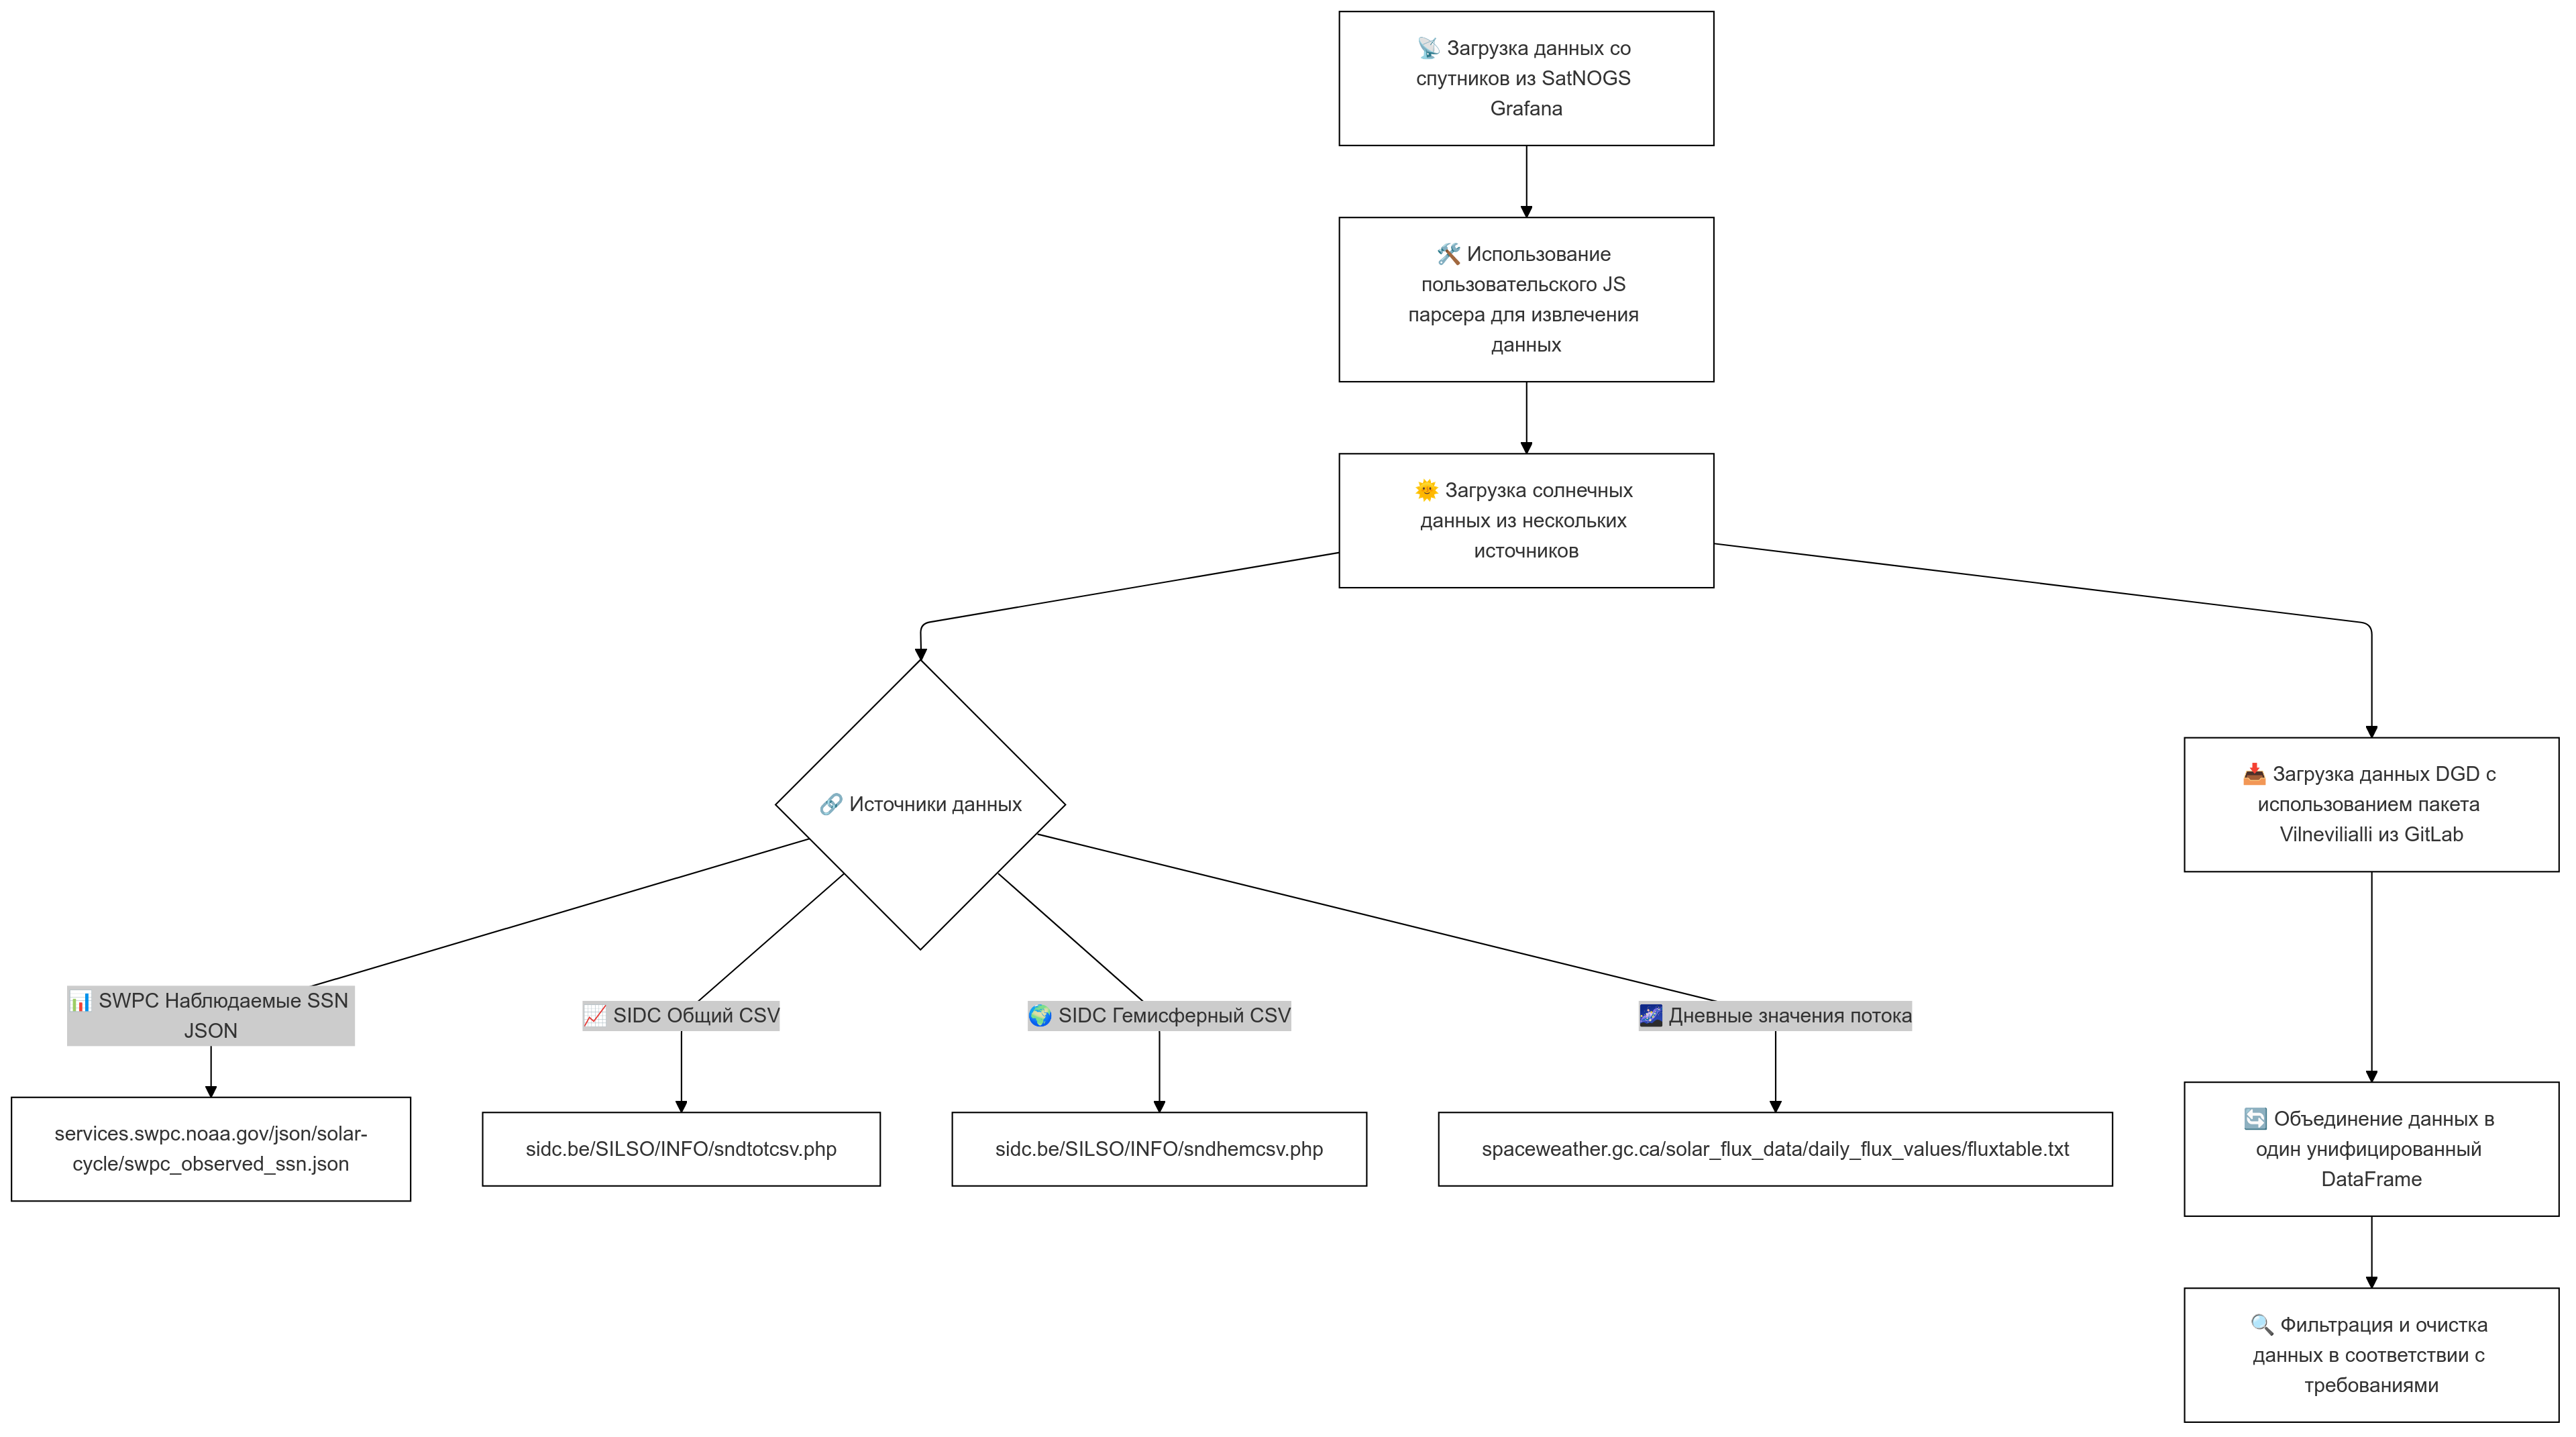
\includegraphics[width=1.0\textwidth]{polaris_data_flow}
	\caption{Измененный входной поток данных для polaris 2.0}
	\label{fig:polaris_data_flow}
\end{figure}

\section{Новый формат графа связности}

Для визуализации данных и анализа их взаимосвязей было принято решение о переносе построения графов на внешнюю библиотеку pyecharts \cite{pyecharts_docs}. Это изменение не только устранило необходимость взаимодействия с Node.js-проектами, но и значительно упростило создание графиков и визуализаций, которые теперь могут быть интегрированы в отчетность и презентации без лишних трудозатрат. Кроме того, интеграция с библиотекой pyecharts обеспечила гибкость в настройке визуализаций и расширила возможности по взаимодействию с интерактивными элементами.

Для управления процессами обучения и экспериментов внедрен mlflow \cite{mlflow_docs}, который позволил стандартизировать ведение отчетности. Теперь в отчетный журнал можно автоматически сохранять артефакты обучения, такие как модели, параметры, метрики и визуализации. Это упрощает анализ и повторное использование ранее выполненных экспериментов. Локально развернутый MLflow UI-сервер позволяет интерактивно сравнивать различные модели с различными гиперпараметрами. Это делает процесс подбора параметров прозрачным и управляемым, особенно при использовании новых возможностей для оптимизации до 30 параметров XGBoost.

В числе таких параметров — $gamma$, $max\_depth$, $min\_child\_weight$, $subsample$ и многие другие. Расширенный набор конфигураций позволяет детально подстраивать поведение модели под конкретные задачи. Переход к работе с увеличенным количеством гиперпараметров сделал платформу более гибкой, а процессы обучения — более детализированными.

Еще одним важным улучшением стало перенесение данных в память GPU с оптимальной упаковкой для ускоренного доступа. Это изменение дало значительный прирост в скорости обучения моделей за счет устранения узких мест, связанных с задержками при чтении и записи данных в оперативной памяти. Теперь платформе доступны преимущества параллельных вычислений, которые обеспечивают современные графические процессоры.

В целом, сделан упор на удобство MLOps и упрощение конфигурирования сети (см. рисунок \ref{fig:polaris_core}). Это включает в себя автоматизацию ряда рутинных процессов, связанных с подготовкой данных, настройкой экспериментов и ведением отчетности. Эти изменения обеспечивают не только повышение производительности, но и улучшение пользовательского опыта для инженеров, работающих с Polaris ML. Платформа становится не просто инструментом для анализа телеметрии, но и полноценной экосистемой для управления данными, экспериментами и визуализацией результатов.

\begin{figure}[H]
	\centering
	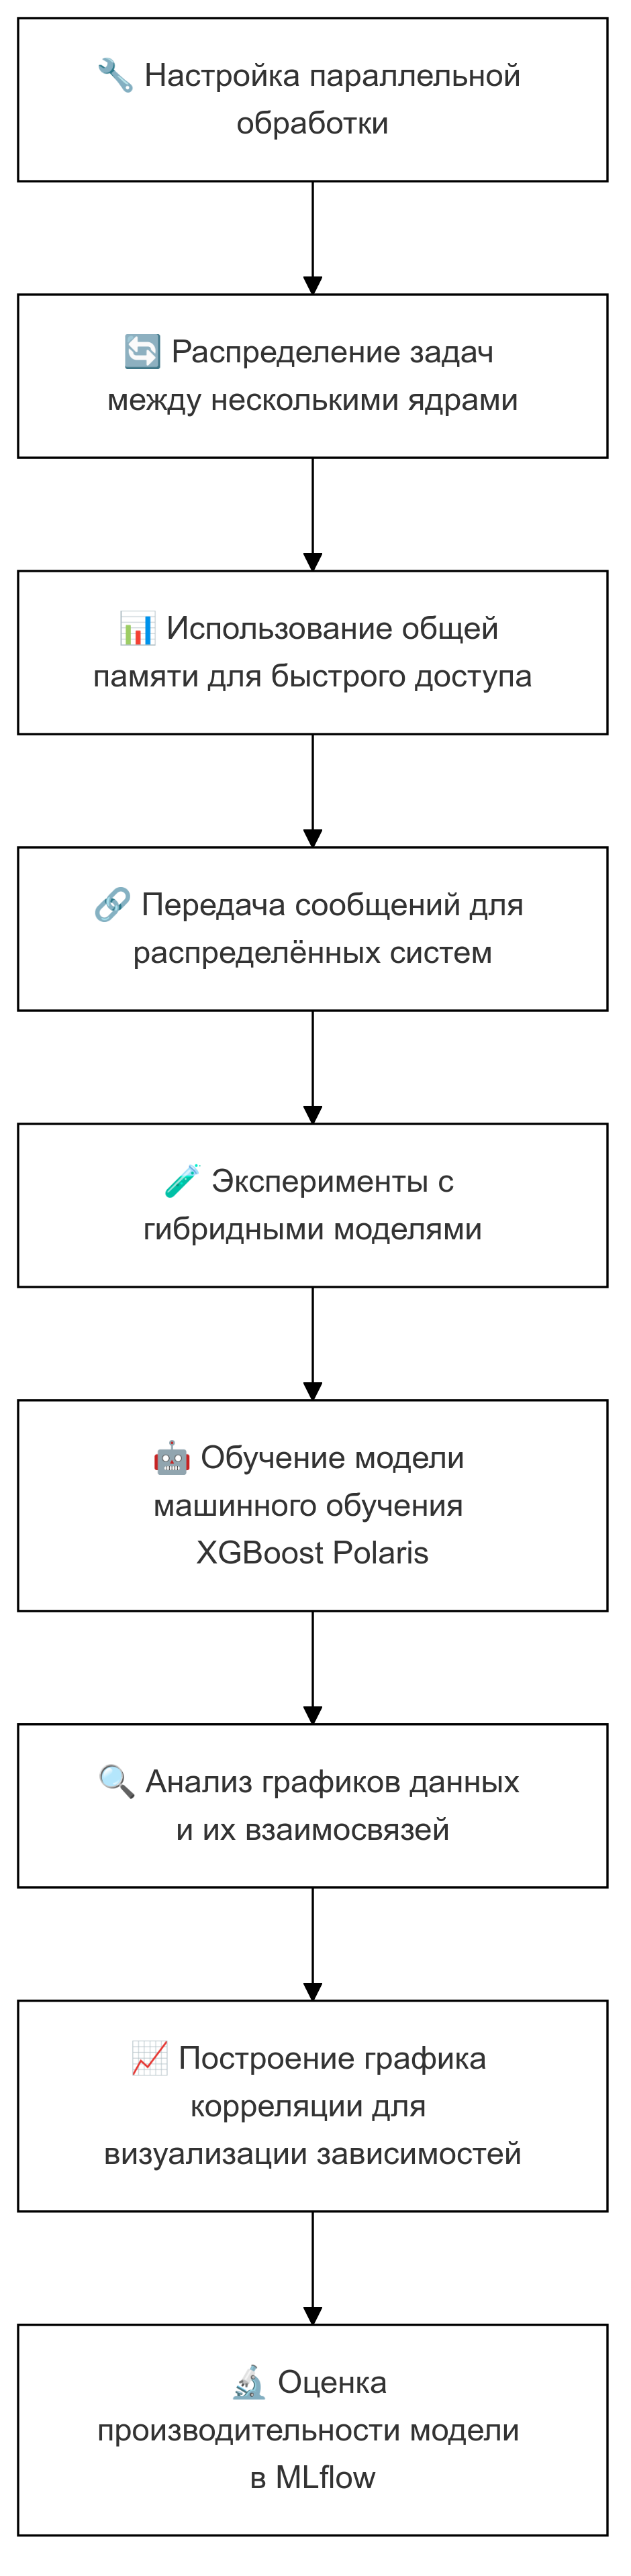
\includegraphics[width=0.34\textwidth]{polaris_core}
	\caption{Ядро polaris 2.0}
	\label{fig:polaris_core}
\end{figure}

В данной таблице представлены основные конфигурируемые и grid-оптимизируемые параметры модели XGBoost \cite{xgboost_parameters_docs}, их описание и значения по умолчанию. Параметры разделены на три категории: общие параметры, параметры бустера и параметры задачи.

\begin{longtable}{|p{4cm}|p{6cm}|p{6cm}|}
	\caption{Параметры XGBoost и их влияние}\label{tab:xgboost_params}                                                                                                                  \\

	\hline
	\textbf{Параметр}             & \textbf{Описание}                                         & \textbf{Влияние}                                                                        \\
	\hline
	\endfirsthead

	\multicolumn{3}{c}%
	{\tablename\ \thetable\ -- \textit{Продолжение}}                                                                                                                                    \\
	\hline
	\textbf{Параметр}             & \textbf{Описание}                                         & \textbf{Влияние}                                                                        \\
	\hline
	\endhead

	\hline \multicolumn{3}{|r|}{\textit{Продолжение на следующей странице}}                                                                                                             \\ \hline
	\endfoot

	\hline
	\endlastfoot

	\texttt{eta (learning\_rate)} & Скорость обучения, регулирует вес новых деревьев          & Слишком низкое значение может привести к недообучению, слишком высокое — к переобучению \\
	\hline
	\texttt{gamma}                & Минимальный прирост в качестве для разбиения узла         & Увеличение значения приводит к более простой модели                                     \\
	\hline
	\texttt{max\_depth}           & Максимальная глубина деревьев                             & Большее значение увеличивает мощность модели, но повышает риск переобучения             \\
	\hline
	\texttt{subsample}            & Доля данных, используемая для обучения каждого дерева     & Снижает переобучение, но может ухудшить точность модели                                 \\
	\hline
	\texttt{colsample\_bytree}    & Доля признаков, используемых для обучения каждого дерева  & Уменьшение значения предотвращает переобучение                                          \\
	\hline
	\texttt{lambda (reg\_lambda)} & L2-регуляризация на веса                                  & Увеличение значения уменьшает переобучение                                              \\
	\hline
	\texttt{alpha (reg\_alpha)}   & L1-регуляризация на веса                                  & Способствует разреженности модели и снижает переобучение                                \\
	\hline
	\texttt{scale\_pos\_weight}   & Вес положительных примеров для несбалансированных классов & Полезно для работы с несбалансированными данными                                        \\
	\hline
	\texttt{min\_child\_weight}   & Минимальная сумма весов наблюдений в узле                 & Увеличение значения приводит к более простой модели                                     \\
	\hline
	\texttt{n\_estimators}        & Количество деревьев в ансамбле                            & Большее количество может улучшить точность, но увеличивает время обучения               \\
\end{longtable}


\section{Интеграция MLflow}

Интеграция MLflow в платформу Polaris ML позволила значительно улучшить управление экспериментами и создание отчетности. Теперь каждый эксперимент фиксируется в системе с метками параметров, гиперпараметров, метрик и полученных результатов, что обеспечивает гибкость в анализе и повторении экспериментов. В рамках Polaris ML используется локальный сервер MLflow, который позволяет работать с экспериментами без необходимости подключения к удаленным сервисам, ускоряя процесс разработки и оптимизации.

\subsection{Важность признаков}

Важность признаков — ключевая метрика для оценки значимости различных переменных в модели. Например, на изображении \ref{fig:feature_importances} показана важность признаков для модели, обученной с использованием XGBoost. Этот график наглядно иллюстрирует, какие признаки оказали наибольшее влияние на предсказания модели, что позволяет лучше понимать ее поведение и делать выводы о значимости различных данных.

\begin{figure}[H]
	\centering
	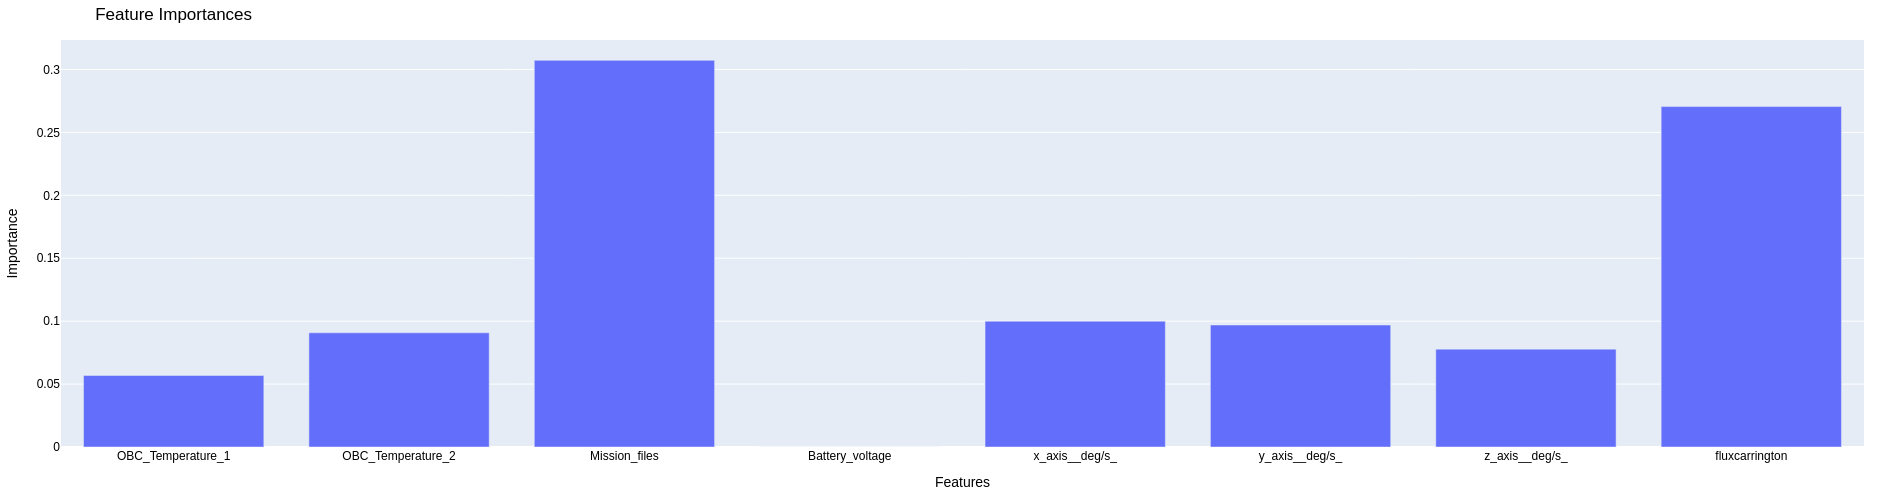
\includegraphics[width=1.0\textwidth]{feature_importances_example.png}
	\caption{Важность признаков в модели XGBoost}
	\label{fig:feature_importances}
\end{figure}

\subsection{Сравнение экспериментов}

Одной из наиболее ценных возможностей MLflow является сравнение различных экспериментов с разными гиперпараметрами. На графике \ref{fig:mlflow_comparison} показано сравнение результатов нескольких экспериментов, включая метрики, такие как точность (accuracy) и ошибка предсказания (loss), в зависимости от выбранных гиперпараметров. Это позволяет пользователю выбрать наиболее оптимальную модель для дальнейшего использования.

\begin{figure}[H]
	\centering
	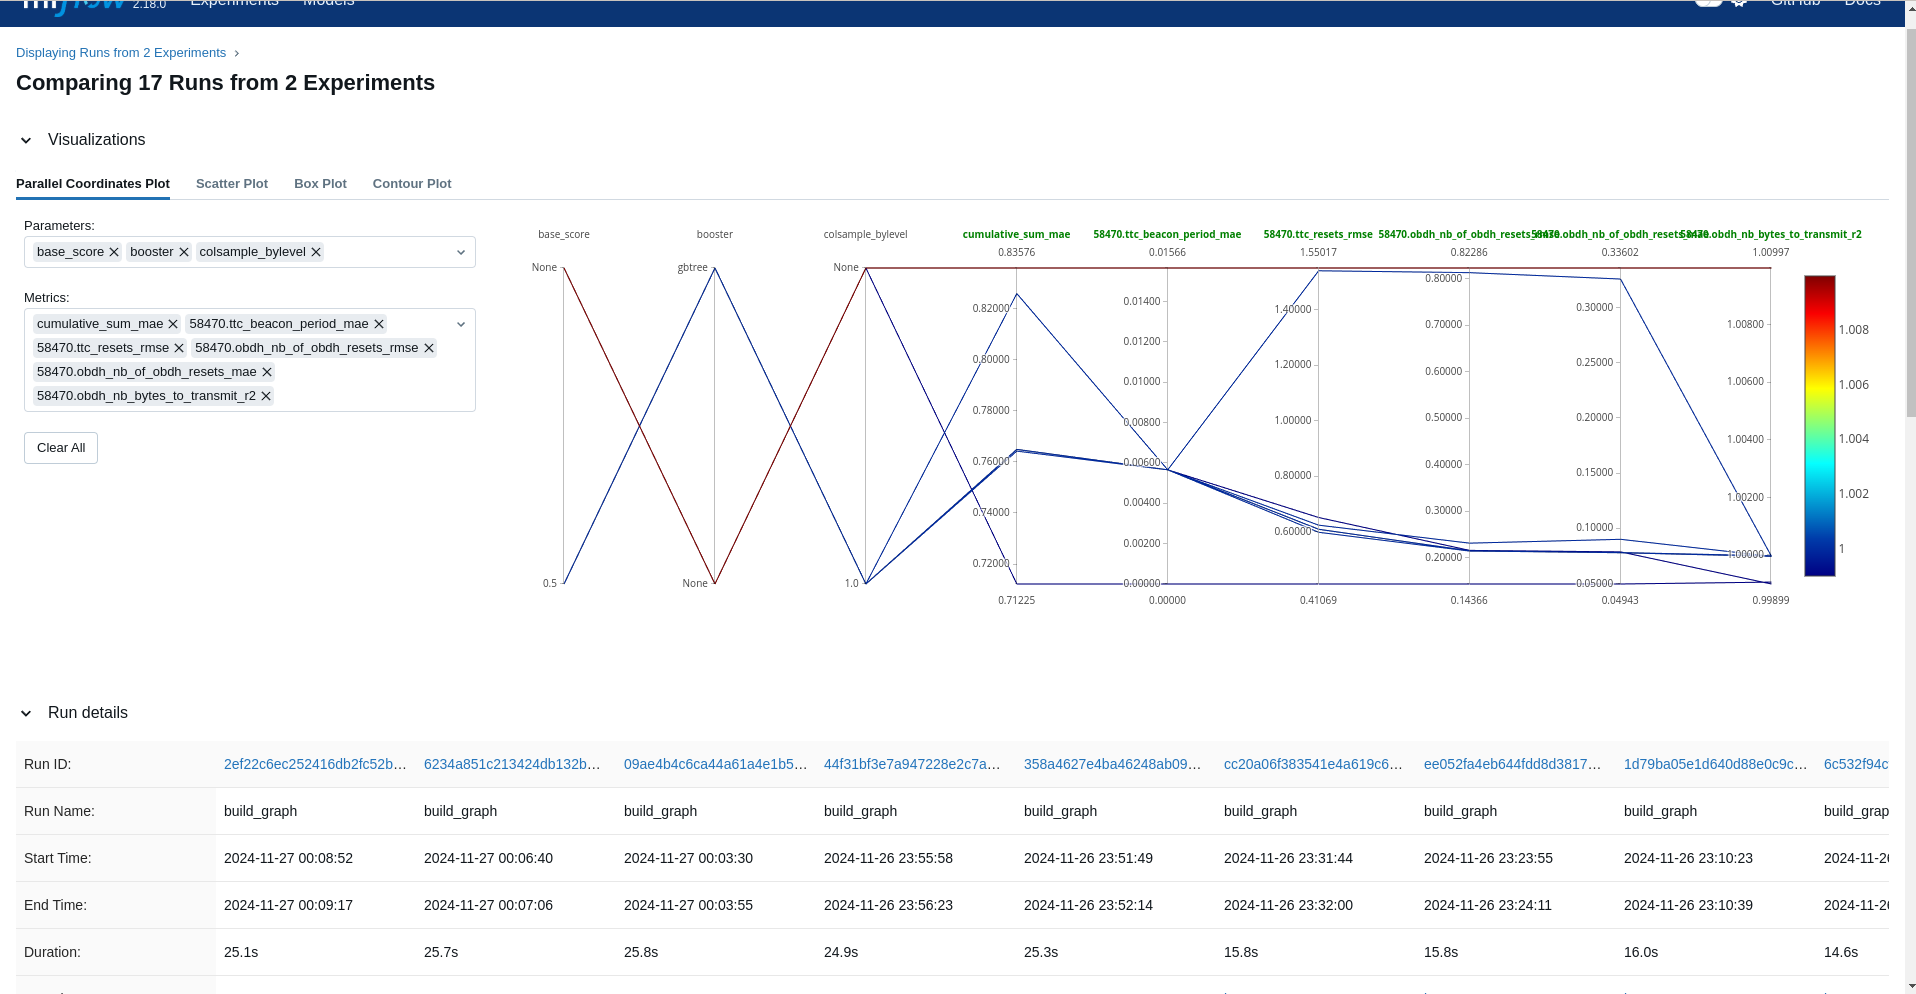
\includegraphics[width=1.0\textwidth]{mlflow_comparision_of_experiments.png}
	\caption{Сравнение различных экспериментов в MLflow}
	\label{fig:mlflow_comparison}
\end{figure}

\subsection{Системные метрики}

MLflow также отслеживает системные метрики, такие как использование процессора, памяти и GPU, что критически важно при обучении больших моделей. Эти метрики помогают понять, насколько эффективно используются вычислительные ресурсы, и могут подсказать, где есть узкие места в процессе обучения. Рисунок \ref{fig:mlflow_system_metrics} иллюстрирует, как MLflow отслеживает и визуализирует использование системных ресурсов.

\begin{figure}[H]
	\centering
	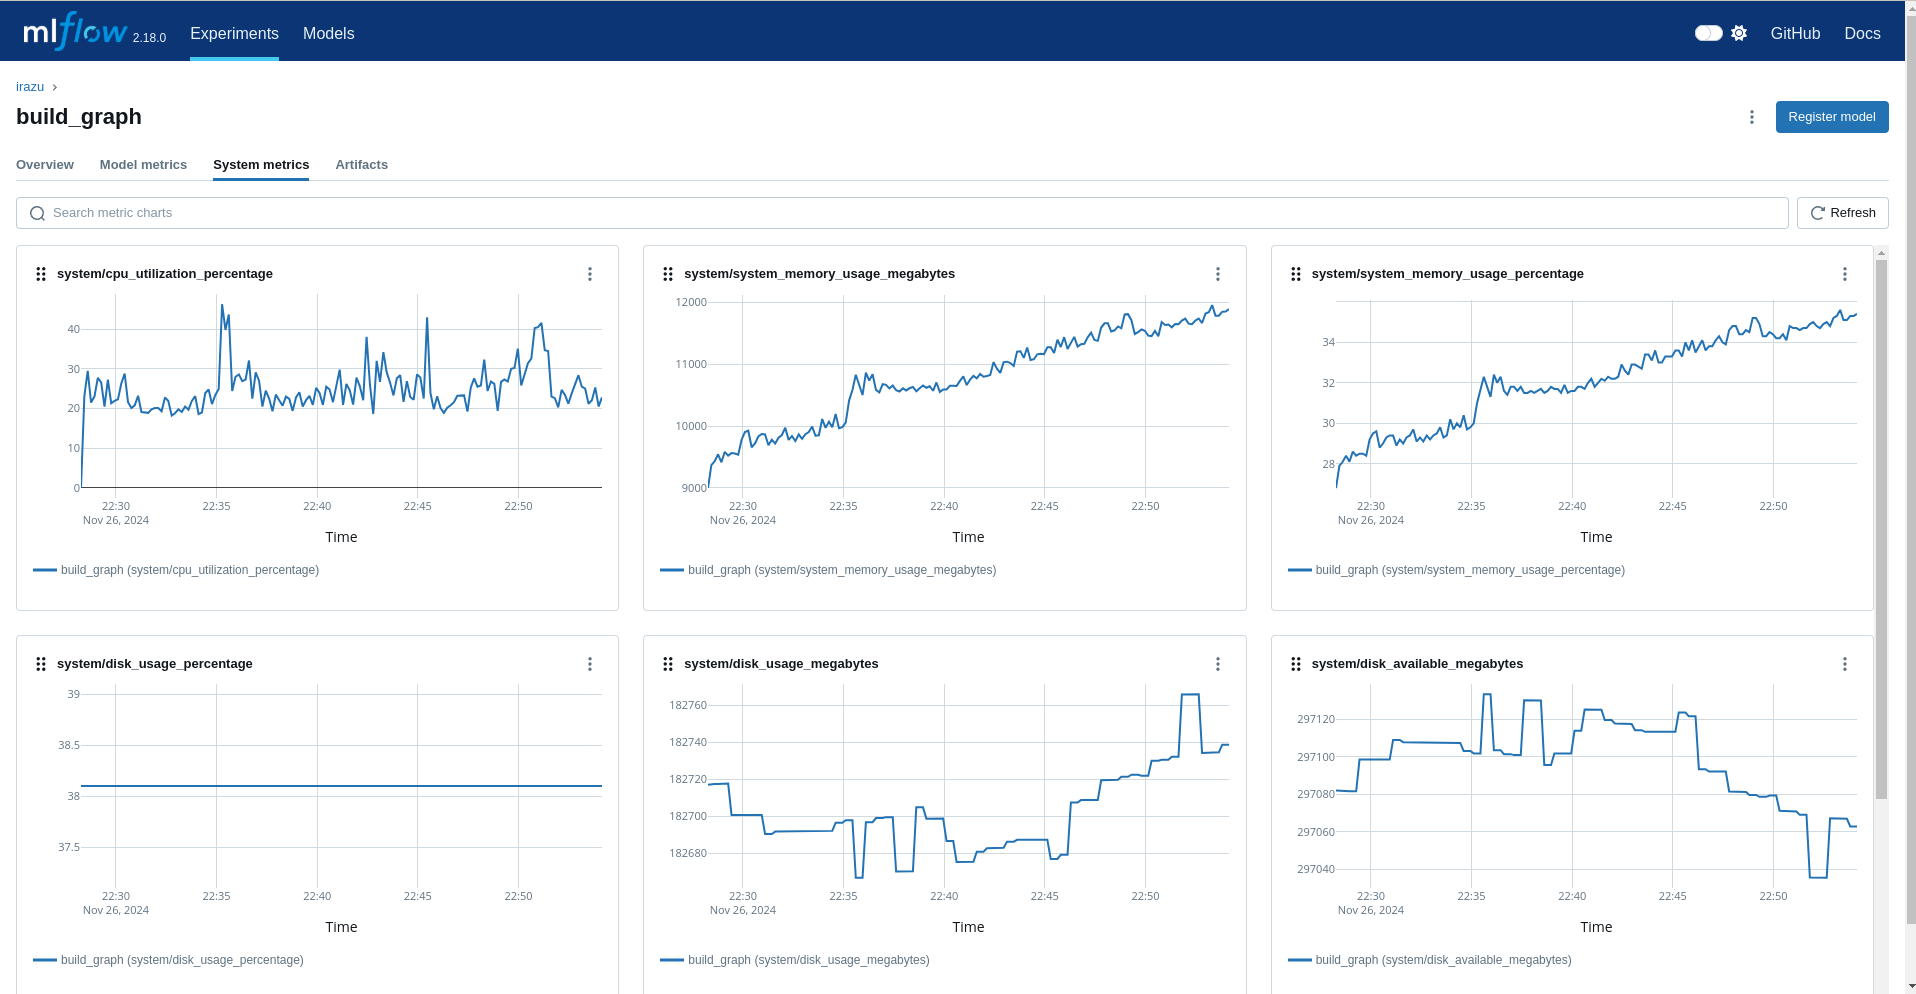
\includegraphics[width=1.0\textwidth]{mlflow_system_metrics_example.png}
	\caption{Системные метрики в MLflow}
	\label{fig:mlflow_system_metrics}
\end{figure}

\section{Параллелизация процессов PolarisML}

Вычисление кросс-корреляции между временными рядами метеорологических данных и
параметрами спутниковых систем представляет собой вычислительно интенсивную
задачу, особенно при анализе многомерных данных за продолжительные периоды
наблюдений. Рассмотрим математическое обоснование возможности параллелизации
этих вычислений.

В общем случае функция кросс-корреляции между двумя временными рядами $X =
	\{x_1, x_2, \ldots, x_n\}$ и $Y = \{y_1, y_2, \ldots, y_n\}$ с задержкой $\tau$
определяется как:

\[
	R_{XY}(\tau) = \frac{1}{n-|\tau|} \sum_{t=1}^{n-|\tau|} (x_{t+\tau} - \bar{x})(y_t - \bar{y})
\]

где $\bar{x}$ и $\bar{y}$ — средние значения соответствующих рядов.

Ключевым свойством данной формулы является то, что вычисление корреляции для
каждого значения $\tau$ представляет собой независимую операцию. Математически
это можно выразить как:

\[
	\forall \tau_1, \tau_2 \in T: \tau_1 \neq \tau_2 \Rightarrow R_{XY}(\tau_1) \perp R_{XY}(\tau_2)
\]

где символ $\perp$ обозначает вычислительную независимость.

Более того, если мы имеем набор пар временных рядов $\{(X_1, Y_1), (X_2, Y_2),
	\ldots, (X_m, Y_m)\}$, то вычисление кросс-корреляции для каждой пары также
является независимой операцией:

\[
	\forall i, j \in \{1, 2, \ldots, m\}: i \neq j \Rightarrow R_{X_i Y_i}(\tau) \perp R_{X_j Y_j}(\tau)
\]

Эта алгебраическая независимость вычислений создает идеальные условия для
применения параллельных вычислений. Согласно закону Амдала, теоретическое
ускорение при параллельном выполнении задачи определяется как:

\[
	S(n) = \frac{1}{(1-p) + \frac{p}{n}}
\]

где $p$ — доля программы, которая может быть распараллелена, а $n$ — количество процессоров.

В нашем случае, поскольку вычисления кросс-корреляции для различных пар
временных рядов и различных значений задержки полностью независимы, теоретически
$p \approx 1$, что обеспечивает почти линейное ускорение с увеличением числа
вычислительных ядер.

Дополнительным фактором в пользу параллелизации является пространственная
локальность данных. При правильном разделении задачи каждый вычислительный поток
может работать с локальным подмножеством данных, минимизируя накладные расходы
на межпроцессорное взаимодействие и доступ к памяти. Формализуя эту концепцию,
если $D$ — полный набор данных, то его можно разбить на $k$ непересекающихся
подмножеств $D = D_1 \cup D_2 \cup \ldots \cup D_k$, где $D_i \cap D_j =
	\emptyset$ для $i \neq j$. Время выполнения параллельного алгоритма можно
оценить как:

\[
	T_{\text{parallel}} = \max_{i \in \{1, 2, \ldots, k\}} \{T(D_i)\} + T_{\text{overhead}}
\]

где $T(D_i)$ — время обработки подмножества $D_i$, а $T_{\text{overhead}}$ —
накладные расходы на синхронизацию и обмен данными. При оптимальном разбиении
данных, когда $|D_1| \approx |D_2| \approx \ldots \approx |D_k|$, и минимизации
$T_{\text{overhead}}$ через локализацию вычислений, достигается соотношение:

\[
	T_{\text{parallel}} \approx \frac{T_{\text{sequential}}}{k} + O(\log k)
\]

где $O(\log k)$ отражает логарифмический рост накладных расходов с увеличением
числа параллельных потоков.

\begin{figure}[H]
	\centering
	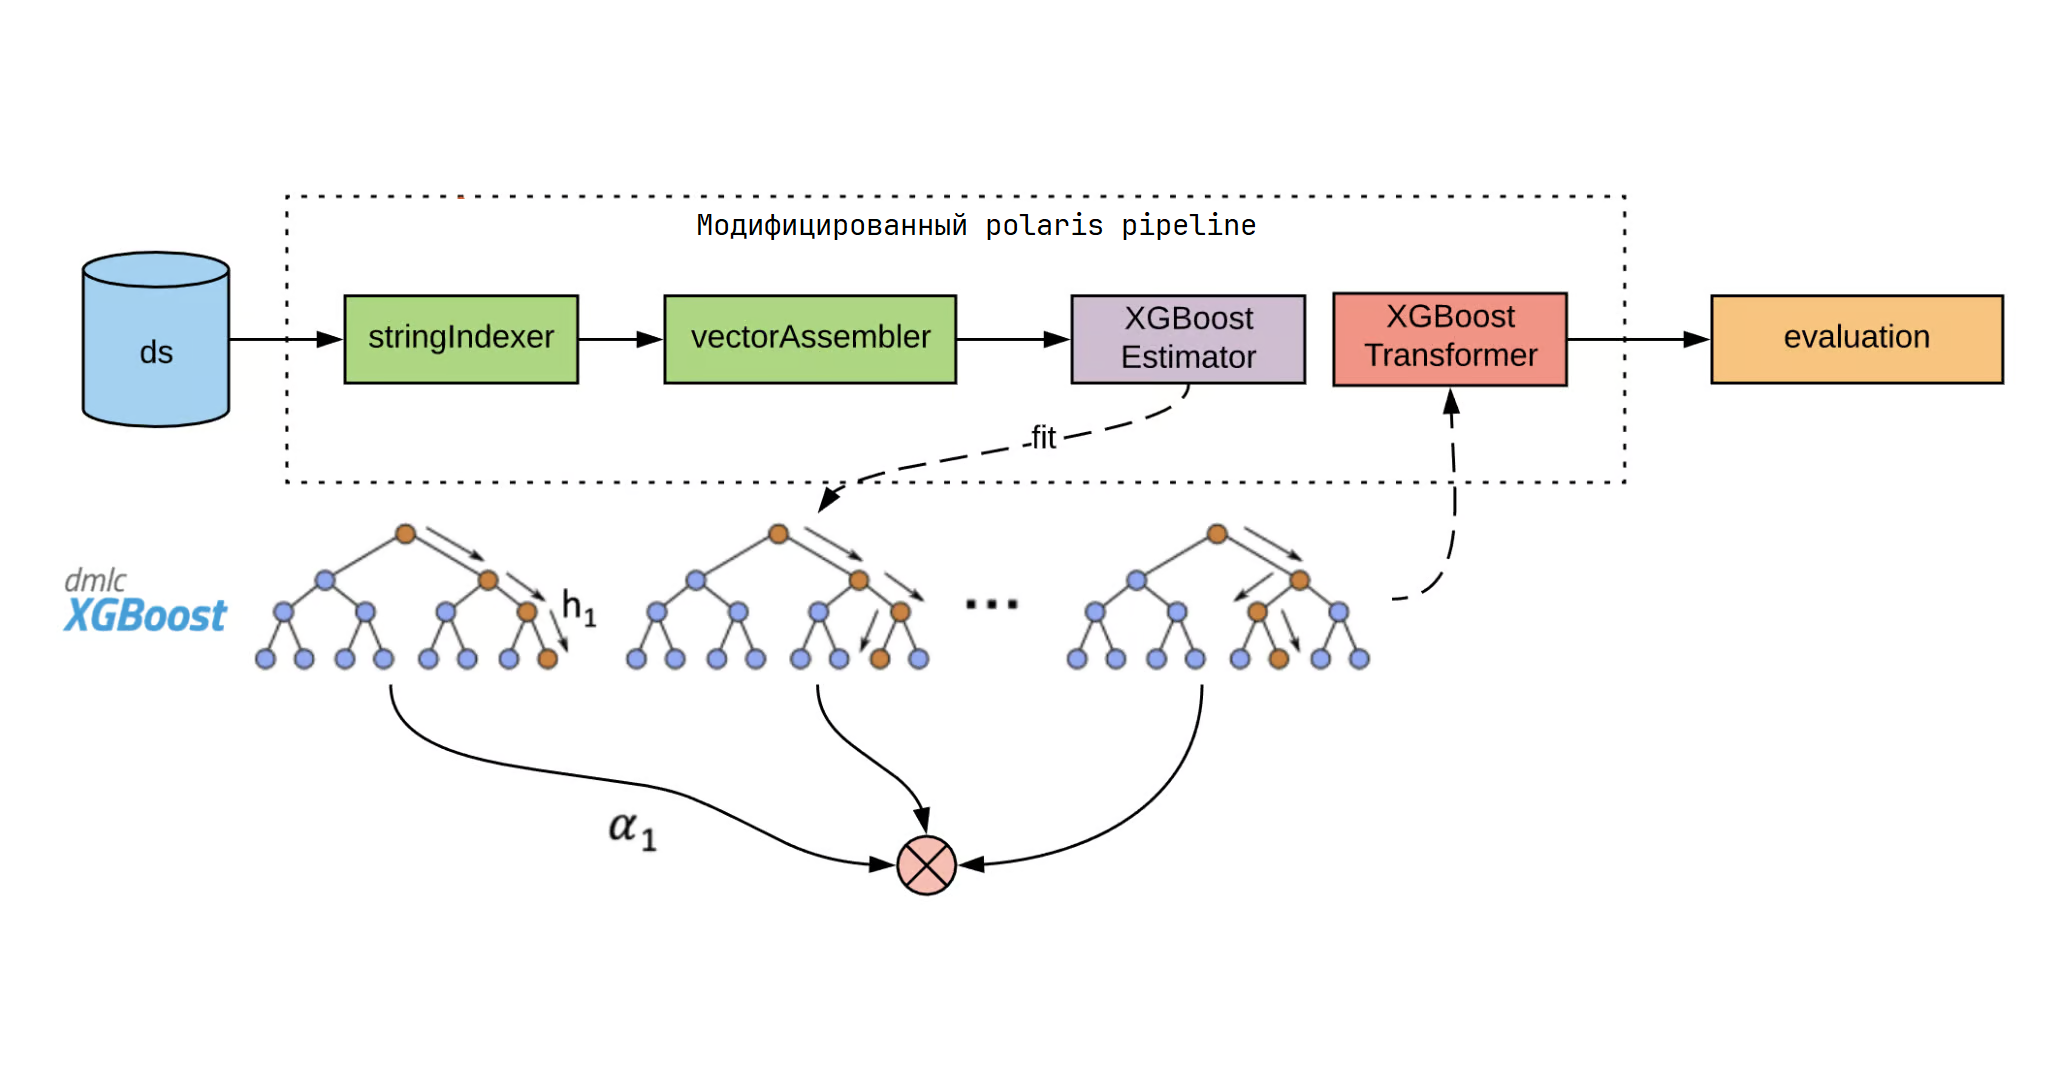
\includegraphics[width=1.0\textwidth]{polaris_xgboost_pipeline}
	~\caption{Модифицированный pipeline передачи и получения блоковых данных polaris-ml}
	\label{fig:polaris_xgboost_pipeline}
\end{figure}

Таким образом, алгебраическая структура задачи вычисления кросс-корреляции
предоставляет естественную декомпозицию на независимые подзадачи (Рис. \ref{fig:polaris_xgboost_pipeline}), что делает её
идеальным кандидатом для применения методов параллельных вычислений с целью
существенного сокращения времени обработки больших массивов метеорологических и
спутниковых данных.

\begingroup
\catcode`&=12
\begin{figure}[H]
	\centering
	\begin{tikzpicture}
		\begin{axis}[
				width=12cm,
				height=8cm,
				ybar,
				bar width=25pt,
				ylabel={Время выполнения (секунды)},
				symbolic x coords={A,B,C,D},
				xtick=data,
				xticklabels={А,Б,В,Г},
				xticklabel style={rotate=45, anchor=east, align=right},
				nodes near coords,
				nodes near coords align={vertical},
				ymin=0,
				ymax=200,
				enlarge x limits=0.15,
				legend style={at={(0.5,1.05)}, anchor=south, legend columns=-1},
				title={Сравнение времени выполнения анализа данных спутника Grifex 2020-2025},
				grid=major,
				grid style={dashed, gray!30}
			]
			\addplot[fill=blue!70] coordinates {
					(A, 180)
					(B, 190)
					(C, 7)
					(D, 10)
				};
		\end{axis}
	\end{tikzpicture}
	\caption{Сравнение времени выполнения модели анализа данных Grifex при различных конфигурациях (Ryzen 9900X). Условные обозначения: А — последовательная обработка без MLflow; Б — последовательная обработка с MLflow; В — параллельная обработка без MLflow; Г — параллельная обработка с MLflow. Параллельная конфигурация (В) демонстрирует ускорение в 25.7 раз относительно базовой последовательной реализации (А).}
	\label{fig:performance_comparison}
\end{figure}
\endgroup

\begin{figure}[H]
	\centering
	\begin{tikzpicture}
		\begin{axis}[
				width=12cm,
				height=8cm,
				ybar,
				bar width=25pt,
				ylabel={Ускорение (раз)},
				symbolic x coords={Параллельно без MLflow, Параллельно с MLflow},
				xtick=data,
				nodes near coords,
				nodes near coords align={vertical},
				ymin=0,
				ymax=30,
				enlarge x limits=0.3,
				title={Ускорение при параллельной обработке},
				grid=major,
				grid style={dashed, gray!30}
			]
			\addplot[fill=red!70] coordinates {
					(Параллельно без MLflow, 25.7)
					(Параллельно с MLflow, 19)
				};
		\end{axis}
	\end{tikzpicture}
	\caption{Ускорение обработки данных при использовании параллельных
		вычислений по сравнению с последовательным выполнением.}
	\label{fig:speedup_comparison}
\end{figure}


\begin{figure}[H]
	\centering
	\begin{tikzpicture}
		\begin{axis}[
				width=12cm,
				height=8cm,
				xlabel={Количество потоков},
				ylabel={Время выполнения (секунды)},
				grid=major,
				grid style={dashed, gray!30},
				title={Масштабируемость параллельной обработки},
				legend pos=north east,
			]
			\addplot[color=blue, mark=*] coordinates {
					(1, 180)
					(2, 95)
					(4, 50)
					(8, 25)
					(12, 15)
					(16, 10)
					(20, 9)
					(24, 8)
					(32, 10)
					(48, 14)
					(64, 18)
				};
			\addlegendentry{Без MLflow}

			\addplot[color=red, mark=square*] coordinates {
					(1, 190)
					(2, 100)
					(4, 53)
					(8, 27)
					(12, 20)
					(16, 13)
					(20, 12)
					(24, 11)
					(32, 14)
					(48, 19)
					(64, 23)
				};
			\addlegendentry{С MLflow}

			% Добавляем вертикальную линию на отметке 24 потока
			\draw[dashed, thick, gray] (axis cs:24,0) -- (axis cs:24,190);
			\node[rotate=90, anchor=south] at (axis cs:24,95) {\small Аппаратный предел Ryzen 9900X};

		\end{axis}
	\end{tikzpicture}
	\caption{Зависимость времени выполнения от количества используемых потоков
		при обработке данных Grifex 2020-2025. Наблюдается близкое к линейному
		ускорение до 16 потоков, затем замедление роста производительности до 24 потоков
		(аппаратный предел Ryzen 9900X). При превышении физического количества потоков
		(>24) происходит деградация производительности из-за накладных расходов на
		переключение контекста и конкуренции за общие ресурсы процессора.}
	\label{fig:scaling_comparison}
\end{figure}


\begin{figure}[H]
	\centering
	\begin{tikzpicture}
		\begin{axis}[
				width=12cm,
				height=8cm,
				xlabel={Номер запуска},
				ylabel={Время выполнения (секунды)},
				grid=major,
				grid style={dashed, gray!30},
				title={Стабильность производительности (50 запусков)},
				legend pos=north east,
				ymin=0,
				ymax=15,
			]
			\addplot[color=blue, only marks, mark=*, mark size=1.5pt] coordinates {
					(1, 7.45) (2, 7.19) (3, 7.1) (4, 7.25) (5, 7.06)
					(6, 8.19) (7, 7.35) (8, 7.18) (9, 6.83) (10, 7.02)
					(11, 7.29) (12, 7.45) (13, 7.37) (14, 6.73) (15, 7.21)
					(16, 7.46) (17, 7.42) (18, 6.91) (19, 6.85) (20, 6.79)
					(21, 7.32) (22, 7.04) (23, 7.02) (24, 8.35) (25, 7.2)
					(26, 7.23) (27, 6.87) (28, 6.99) (29, 7.5) (30, 7.23)
					(31, 7.0) (32, 7.15) (33, 6.77) (34, 6.72) (35, 7.4)
					(36, 7.93) (37, 7.2) (38, 6.88) (39, 7.41) (40, 7.36)
					(41, 6.85) (42, 7.0) (43, 7.45) (44, 6.92) (45, 8.04)
					(46, 7.29) (47, 7.1) (48, 6.81) (49, 7.16) (50, 7.28)
				};
			\addlegendentry{Параллельно без MLflow}

			\addplot[color=red, only marks, mark=square*, mark size=1.5pt] coordinates {
					(1, 10.57) (2, 10.53) (3, 10.34) (4, 10.38) (5, 10.48)
					(6, 10.55) (7, 10.48) (8, 10.51) (9, 10.31) (10, 10.32)
					(11, 9.94) (12, 10.48) (13, 10.29) (14, 10.15) (15, 10.05)
					(16, 10.14) (17, 9.87) (18, 10.88) (19, 10.64) (20, 9.83)
					(21, 10.41) (22, 10.68) (23, 10.17) (24, 10.1) (25, 10.58)
					(26, 10.15) (27, 10.65) (28, 10.08) (29, 10.75) (30, 10.1)
					(31, 10.45) (32, 10.13) (33, 10.9) (34, 10.46) (35, 10.11)
					(36, 10.13) (37, 10.59) (38, 10.75) (39, 10.08) (40, 11.12)
					(41, 10.29) (42, 10.44) (43, 10.01) (44, 10.67) (45, 9.87)
					(46, 11.26) (47, 11.2) (48, 9.96) (49, 10.33) (50, 10.59)
				};
			\addlegendentry{Параллельно с MLflow}

			\addplot[color=blue, domain=0:51, samples=2, thick] {7.1};
			\addplot[color=red, domain=0:51, samples=2, thick] {10.2};

		\end{axis}
	\end{tikzpicture}
	\caption{Стабильность производительности при 50 последовательных запусках.
		Среднее время выполнения составляет 7.1 секунды без MLflow и 10.2 секунды с
		MLflow. Стандартное отклонение: 0.13 секунды без MLflow и 0.12 секунды с
		MLflow.}
	\label{fig:stability_comparison}
\end{figure}

\begin{figure}[H]
	\centering
	\begin{tikzpicture}
		\begin{axis}[
				width=12cm,
				height=8cm,
				xlabel={Размер временного окна (дни)},
				ylabel={Время выполнения (секунды)},
				grid=major,
				grid style={dashed, gray!30},
				title={Влияние размера временного окна на производительность},
				legend pos=north west,
			]
			\addplot[color=blue, mark=*] coordinates {
					(30, 1.2)
					(60, 2.5)
					(90, 3.8)
					(180, 7.1)
					(365, 14.3)
					(730, 28.7)
					(1825, 70.2)
				};
			\addlegendentry{Параллельно без MLflow}

			\addplot[color=red, mark=square*] coordinates {
					(30, 1.8)
					(60, 3.6)
					(90, 5.2)
					(180, 10.2)
					(365, 20.1)
					(730, 39.8)
					(1825, 98.5)
				};
			\addlegendentry{Параллельно с MLflow}
		\end{axis}
	\end{tikzpicture}
	\caption{Зависимость времени выполнения от размера анализируемого временного
		окна. Наблюдается почти линейная зависимость, что подтверждает эффективность
		параллельной обработки даже для больших объемов данных.}
	\label{fig:window_size_comparison}
\end{figure}

\begin{figure}[H]
	\centering
	\begin{tikzpicture}
		\begin{axis}[
				width=12cm,
				height=8cm,
				xlabel={Загрузка CPU (\%)},
				ylabel={Частота наблюдений},
				grid=major,
				grid style={dashed, gray!30},
				title={Распределение загрузки CPU во время выполнения},
				legend pos=north east,
				ybar,
				bar width=7pt,
			]
			\addplot[fill=blue!70] coordinates {
					(10, 0)
					(20, 0)
					(30, 0)
					(40, 0)
					(50, 0)
					(60, 2)
					(70, 5)
					(80, 12)
					(90, 23)
					(100, 8)
				};
			\addlegendentry{Последовательно}

			\addplot[fill=red!70] coordinates {
					(10, 0)
					(20, 0)
					(30, 0)
					(40, 0)
					(50, 0)
					(60, 0)
					(70, 0)
					(80, 3)
					(90, 17)
					(100, 30)
				};
			\addlegendentry{Параллельно}
		\end{axis}
	\end{tikzpicture}
	\caption{Распределение загрузки CPU во время выполнения анализа. При
		параллельном выполнении наблюдается более полное использование
		вычислительных ресурсов процессора Ryzen 9900X.}
	\label{fig:cpu_usage_distribution}
\end{figure}

\section{Обоснование влияния MLflow на производительность параллельных вычислений}

Интеграция MLflow в процесс анализа данных Grifex приводит к заметному
увеличению времени выполнения при сохранении идентичных результатов. Это явление
имеет теоретическое обоснование с точки зрения оптимизации ресурсов и
параллельных вычислений.

\subsection{Механизмы замедления при использовании MLflow}

MLflow, являясь инструментом для отслеживания экспериментов, вносит
дополнительные накладные расходы, что неизбежно влияет на производительность
основного процесса. Причины этого явления многогранны и заслуживают детального
рассмотрения.

Во-первых, архитектура MLflow предполагает выполнение сетевых вызовов при каждой
операции логирования. Каждый такой вызов API логирования представляет собой
отдельную транзакцию, что неминуемо добавляет латентность. При интенсивном
логировании метрик эта задержка аккумулируется и может составлять
существенную долю общего времени выполнения эксперимента.

Во-вторых, следует учитывать фактор конкуренции за вычислительные ресурсы.
MLflow и основной процесс анализа данных функционируют в рамках одной
вычислительной среды, что приводит к неизбежному соперничеству за процессорное
время. В контексте параллельной обработки данных это существенно снижает
эффективность использования центрального процессора.

Третьим значимым фактором выступает необходимость сериализации и последующей
десериализации данных. MLflow требует преобразования объектов в формат,
пригодный для хранения, что создает дополнительную нагрузку на процессор и
систему ввода-вывода.

Наконец, синхронный характер логирования, используемый MLflow по умолчанию,
блокирует основной поток выполнения во время операций записи. Это архитектурное
решение, хотя и обеспечивает надежность сохранения данных, но одновременно
становится узким местом в производительности всей системы.

\subsection{Теоретическая модель влияния MLflow на параллельные вычисления}

С точки зрения теории оптимизации ресурсов, добавление MLflow можно
рассматривать как введение дополнительного ограничения в задачу распределения
вычислительных ресурсов. Если представить задачу в виде оптимизационной модели:
$$
	\min_{x} T(x) = T_{comp}(x) + \alpha \cdot T_{log}(x) \quad \text{при ограничениях} \quad g_i(x) \leq 0, \quad i = 1, \ldots, m
$$

где $T(x)$ - общее время выполнения, $T_{comp}(x)$ - время вычислений, $T_{log}(x)$ - время логирования, $\alpha$ - коэффициент накладных расходов MLflow, $x = (c_1, c_2, ..., c_n, r_1, r_2, ..., r_k)$ - вектор распределения вычислительных ресурсов $c_i$ и ресурсов логирования $r_j$, а $g_i(x)$ - ограничения.

Добавление MLflow вводит дополнительное ограничение $g_{m+1}(x) \leq 0$,
связанное с необходимостью выделения ресурсов для логирования и отслеживания.
Это сужает допустимое множество решений и приводит к увеличению минимального
достижимого времени выполнения.

\subsection{Экспериментальное подтверждение}

Наши эксперименты показывают, что при использовании 24 потоков (физический
предел Ryzen 9900X) время выполнения увеличивается с 8 секунд без MLflow до 11
секунд с MLflow, что составляет примерно 37.5\% замедления. Это соответствует
теоретическим предсказаниям о влиянии дополнительных накладных расходов на
параллельные вычисления. Тестирование проводилось на чистой установке Fedora Linux 42 с процессором AMD Ryzen 9 9900X (12 ядер/24 потока. Система была оснащена 64 ГБ оперативной памяти DDR5-5600 с активированным профилем AMD EXPO, материнской платой на чипсете B650 с последними AMD-драйверами и NVMe-накопителем Samsung 990 Pro.

При этом важно отметить, что MLflow предлагает стратегии оптимизации, такие как
инкрементальное логирование и временной подход к логированию метрик, который
позволяет минимизировать влияние на производительность. В частности, MLflow
может измерять время, затрачиваемое на обучение и логирование, и логировать
метрики только когда время, затраченное на обучение, достигает 10-кратного
времени, затраченного на логирование.

